%%%%%%%%%%%%%%%%%%%%%%%%%%%%%%%%%%%%%%%%%%%%%%%%%%%%%%%%%%
%   Autoren:
%   Prof. Dr. Bernhard Drabant
%   Prof. Dr. Dennis Pfisterer
%   Prof. Dr. Julian Reichwald
%%%%%%%%%%%%%%%%%%%%%%%%%%%%%%%%%%%%%%%%%%%%%%%%%%%%%%%%%%

%%%%%%%%%%%%%%%%%%%%%%%%%%%%%%%%%%%%%%%%%%%%%%%%%%%%%%%%%%
%	ANLEITUNG: 
%   1. Ersetzen Sie firmenlogo.jpg im Verzeichnis img
%   2. Passen Sie alle Stellen im Dokument an, die mit 
%      @stud 
%      markiert sind
%%%%%%%%%%%%%%%%%%%%%%%%%%%%%%%%%%%%%%%%%%%%%%%%%%%%%%%%%%

%%%%%%%%%%%%%%%%%%%%%%%%%%%%%%%%%%%%%%%%%%%%%%%%%%%%%%%%%%
%	ACHTUNG: 
%   Für das Erstellen des Literaturverzeichnisses wird das 
%   modernere Paket biblatex in Kombination mit biber 
%   verwendet - nicht mehr das ältere Paket BibTex!
%
%   Bitte stellen Sie Ihre TeX-Umgebung entsprechend ein (z.B. TeXStudio): 
%   Einstellungen --> Erzeugen --> Standard Bibliographieprogramm: biber
%%%%%%%%%%%%%%%%%%%%%%%%%%%%%%%%%%%%%%%%%%%%%%%%%%%%%%%%%%

\documentclass[fontsize=12pt,BCOR=5mm,DIV=12,parskip=half,listof=totoc,
               paper=a4,toc=bibliography,pointlessnumbers]{scrreprt}
               
               %toc=listof,listof=entryprefix,
               
\makeindex

%% Elementare Pakete, Konfigurationen und Definitionen werden geladen (gegebenenfalls anpassen)
% !TEX root =  master.tex

%%%%%%%%%%%%%%%%%%%%%%%%%%%%%%%%%%%%%%%%%%%%%%%%%%%%%%%%%%%%%%%%%%
%	ANLEITUNG: 
% Passen Sie gegebenenfalls alle Stellen im Dokument an, die mit 
% @stud 
% markiert sind.
%%%%%%%%%%%%%%%%%%%%%%%%%%%%%%%%%%%%%%%%%%%%%%%%%%%%%%%%%%%%%%%%%%

\usepackage{makeidx}                  % allows index generation
\usepackage{listings}	                %Format Listings properly
\usepackage{lipsum}                   % Blindtext
\usepackage{graphicx}                 % use various graphics formats
\usepackage{float}
\usepackage[german]{varioref}         % nicer references \vref
\usepackage{caption}	                % better Captions
\usepackage{booktabs}                 % nicer Tabs
\usepackage[hidelinks=true]{hyperref} % keine roten Markierungen bei Links
\usepackage{fnpct}                    % Correct superscripts 
\usepackage{calc}                     % Used for extra space below footsepline, in particular
\usepackage{array}
\usepackage{acronym}
\usepackage{algorithm}
\usepackage{algpseudocode}
\usepackage{setspace}
\usepackage{tocloft}

%% Schriftarten- und Zeichenpakete
\usepackage[T1]{fontenc}
\usepackage[utf8]{inputenc}

%%
%% @stud
%%
%%	FONT SELECTION: Schriftarten und Schriftfamilie
%%%%%%%%%%%%%
%% SCHRIFTART
%%%%%%%%%%%%%
% 0) without decomment: normal font families 
% ...
% 1) Latin Modern 
%\usepackage{lmodern}        
% 2) Times 
%\usepackage{mathptmx}         
% 3) Helvetica
%\usepackage[scaled=.92]{helvet} 
%%%%%%%%%%%%%%%%%%
%%	SCHRIFTFAMILIE
%%%%%%%%%%%%%%%%%%
% ohne Serifen
\renewcommand*{\familydefault}{\sfdefault}
\addtokomafont{disposition}{\sffamily}
%
% mit Serifen
%\renewcommand*{\familydefault}{\rmdefault}
%\addtokomafont{disposition}{\rmfamily}
%
% Typewriter
%\renewcommand*{\familydefault}{\ttdefault}
%\addtokomafont{disposition}{\ttfamily}

%%
%% @stud
%%
%% LANGUAGE SETTINGS
\usepackage[ngerman]{babel} 	        % german language
\usepackage[german=quotes]{csquotes} 	% correct quoting using \enquote{}
%\usepackage[english]{babel}          % english language
%\usepackage{csquotes} 	              % correct quoting using \enquote{}

%%
%% @stud
%%
%% Uncomment the following lines to support hard URL breaks in bibliography 
%\apptocmd{\UrlBreaks}{\do\f\do\m}{}{}
%\setcounter{biburllcpenalty}{9000}% Kleinbuchstaben
%\setcounter{biburlucpenalty}{9000}% Großbuchstaben

%%
%% @stud
%%
%% FOOTNOTES: Count footnotes over chapters
%% \counterwithout{footnote}{chapter}

%	ACRONYMS
\makeatletter
\@ifpackagelater{acronym}{2015/03/20}
{\renewcommand*{\aclabelfont}[1]{\textbf{{\acsfont{#1}}}}}{}
\makeatother

%	LISTINGS
% @stud: ggf. Namen/Text anpassen (englisch)
\renewcommand{\lstlistingname}{Quelltext} 
\renewcommand{\lstlistlistingname}{Quelltextverzeichnis}
\lstset{numbers=left,
	numberstyle=\tiny,
	captionpos=b,
	basicstyle=\ttfamily\small}

%	ALGORITHMS
% @stud: ggf. Namen/Text anpassen (englisch)
\renewcommand{\listalgorithmname}{Algorithmenverzeichnis}
\floatname{algorithm}{Algorithmus}

%	PAGE HEADER / FOOTER
%	Warning: There are some redefinitions throughout the master.tex-file!  DON'T CHANGE THESE REDEFINITIONS!
\RequirePackage[automark]{scrlayer-scrpage}
%alternatively with separation lines: \RequirePackage[automark,headsepline,footsepline]{scrlayer-scrpage}

\renewcommand{\chaptermarkformat}{}
\RedeclareSectionCommand[beforeskip=0pt]{chapter}
\clearscrheadfoot

%\ifoot[\rule{0pt}{\ht\strutbox+\dp\strutbox}DHBW Mannheim]{\rule{0pt}{\ht\strutbox+\dp\strutbox}DHBW Mannheim}
\ofoot[\rule{0pt}{\ht\strutbox+\dp\strutbox}\pagemark]{\rule{0pt}{\ht\strutbox+\dp\strutbox}\pagemark}
\ohead{\headmark}

\newcommand{\TitelDerArbeit}[1]{\def\DerTitelDerArbeit{#1}\hypersetup{pdftitle={#1}}}
\newcommand{\AutorDerArbeit}[1]{\def\DerAutorDerArbeit{#1}\hypersetup{pdfauthor={#1}}}
\newcommand{\Firma}[1]{\def\DerNameDerFirma{#1}}
\newcommand{\Kurs}[1]{\def\DieKursbezeichnung{#1}}
\newcommand{\Abteilung}[1]{\def\DerNameDerAbteilung{#1}}
\newcommand{\Studiengangsleiter}[1]{\def\DerStudiengangsleiter{#1}}
\newcommand{\WissBetreuer}[1]{\def\DerWissBetreuer{#1}}
\newcommand{\FirmenBetreuer}[1]{\def\DerFirmenBetreuer{#1}}
\newcommand{\Bearbeitungszeitraum}[1]{\def\DerBearbeitungszeitraum{#1}}
\newcommand{\Abgabedatum}[1]{\def\DasAbgabedatum{#1}}
\newcommand{\Matrikelnummer}[1]{\def\DieMatrikelnummer{#1}}
\newcommand{\Studienrichtung}[1]{\def\DieStudienrichtung{#1}}
\newcommand{\ArtDerArbeit}[1]{\def\DieArtDerArbeit{#1}}
\newcommand{\Literaturverzeichnis}{Literaturverzeichnis}

\newcommand{\settingBibFootnoteCite}{
	\setlength{\bibparsep}{\parskip}		  % Add some space between biblatex entries in the bibliography
	\addbibresource{bibliography.bib}	    % Add file bibliography.bib as biblatex resource
	\DefineBibliographyStrings{ngerman}{andothers = {{et\,al\adddot}},}
}

\newcommand{\setTitlepage}{
	% !TEX root =  master.tex
% @stud: ggf. Namen/Text anpassen (englisch)
\begin{titlepage}
\begin{minipage}{\textwidth}
		\vspace{-2cm}
		\noindent 
\includegraphics[scale=0.3]{\imagedir/AtosLogo.png} \hfill 
		
\includegraphics{\imagedir/logo.jpg}
\end{minipage}
\vspace{1em}
%\sffamily
\begin{center}
	{\textsf{\large Duale Hochschule Baden-W\"urttemberg Mannheim}}\\[4em]
	{\textsf{\textbf{\large{Projektarbeit}}}}\\[6mm]
	{\textsf{\textbf{\Large{}Automatisierte Erkennung und Ausnutzung von Schwachstellen in Web-Applikationen
	}}} \\[1.5cm]
	{\textsf{\textbf{\large{}Studiengang Informatik}}\\[6mm]
	\textsf{\textbf{Studienrichtung Angewandte Informatik}}}\vspace{10em}
	
	\begin{minipage}{\textwidth}
		\begin{tabbing}
		Wissenschaftliche(r) Betreuer(in): \hspace{0.85cm}\=\kill
		Verfasser: \> Joel Dag \\[1.5mm]
		Matrikelnummer: \> 4811224 \\[1.5mm]
		Firma: \> Atos Information Technology GmbH  \\[1.5mm]
		Kurs: \> TINF21 AI1  \\[1.5mm]
		Studiengangsleiter: \> Prof. Dr. Holger Hofmann \\[1.5mm]
		Abgabedatum: \> 06.10.2022\\[1.5mm]
		Bearbeitungszeitraum: \> 03.01.2022 - 06.10.2022\\[1.5mm]
		Firmenbetreuer: \> Daniel von Schierstedt \\[1.5mm] \\ \\
		Unterschrift Betreuer: \> \underline {\hspace{4cm}}\\[1.5mm] 
%		Eingereicht: \> \DasAbgabedatum	
		\end{tabbing}
	\end{minipage}
\end{center}
\end{titlepage}
	\pagenumbering{roman} % Römische Seitennummerierung
	\normalfont	
}

\newcommand{\initializeText}{
	\clearpage
	\ihead{\chaptername~\thechapter} % Neue Header-Definition
	\pagenumbering{arabic}           % Arabische Seitenzahlen
}

\newcommand{\initializeBibliography}{
	\ihead{}
	\printbibliography[title=\Literaturverzeichnis] 
	\cleardoublepage
}

\newcommand{\initializeAppendix}{
	\appendix
  \ihead{}
  \cftaddtitleline{toc}{chapter}{Anhang}{}
}



%%
%% @stud
%%
%% PERSÖNLICHE ANGABEN (BITTE VOLLSTÄNDIG EINGEBEN zwischen den Klammern: {...})
%%
\ArtDerArbeit{<Projekt>} % "Bachelor" oder "Projekt" wählen
\TitelDerArbeit{<Konzeptentwicklung und Implementierung einer Pausenfunktion für den T4TC-Runner>}
\AutorDerArbeit{<Joel Dag>}
\Abteilung{<Product Lifecycle Management Paderborn>}
\Firma{<Atos Information Technology GmbH>}
\Kurs{<TINF21 AI1>}
\Studienrichtung{<Angewandte Informatik>}
\Matrikelnummer{<4811224>}
\Studiengangsleiter{<Prof. Dr. Holger Hofmann>}
\WissBetreuer{<Ihr(e) wissenschaftliche(r) Betreuer(in)>}
\FirmenBetreuer{<Simon Sonnenkemper>}
\Bearbeitungszeitraum{dd.mm.yyyy -- DD.MM.YYYY}
\Abgabedatum{dd.mm.yyyy}

%%
%% @stud
%%
%% BIBLIOGRAPHY (@stud: Bibliographie-Stil wählen - Position und Indizierung)
%%  Auswahl zwischen: 
%%   NUMERIC Style
%%   IEEE Style
%%   ALPHABETIC Style
%%   HARVARD Style
%%   CHICAGO Style 
%%   (oder eigenen zulässigen Stil wählen) 
%%
%%%%%%%%%%%%%
%% Zitierstil
%%%%%%%%%%%%%
% NUMERIC Style - e. g. [12]
%\newcommand{\indextype}{numeric} 
%
% IEEE Style - numeric kind of style 
%\newcommand{\indextype}{ieee} 
%
% ALPHABETIC Style - e. g. [AB12]
\newcommand{\indextype}{alphabetic} 
%
% HARVARD Style 
%\newcommand{\indextype}{apa} 
%
% CHICAGO Style 
%\newcommand{\indextype}{authoryear}
%
%%%%%%%%%%%%%%%%%%%%%%
%% Position des Zitats
%%%%%%%%%%%%%%%%%%%%%%
\newcommand{\position}{inline} 
%
% (!!) FOOTNOTE POSITION NOT RECOMMENDED IN MINT DOMAIN:
%\newcommand{\position}{footnote}

%% Final: Setzen des Zitierstils und der Zitatposition
\usepackage[backend=biber, autocite=\position, style=\indextype]{biblatex} 	
\settingBibFootnoteCite

%%
%% Definitionen und Commands
%%
\newcommand{\abs}{\par\vskip 0.2cm\goodbreak\noindent}
\newcommand{\nl}{\par\noindent}
\newcommand{\mcl}[1]{\mathcal{#1}}
\newcommand{\nowrite}[1]{}
\newcommand{\NN}{{\mathbb N}}
\newcommand{\imagedir}{img}

\makeindex

\begin{document}

\setTitlepage
%% !TEX root =  master.tex
% @stud: ggf. Namen/Text anpassen (englisch)
\begin{titlepage}
	\begin{minipage}{\textwidth}
		\vspace{-2cm}
		\noindent 
\includegraphics[scale=0.3]{\imagedir/AtosLogo.png} \hfill 
		
\includegraphics{\imagedir/logo.jpg}
	\end{minipage}
	\vspace{1em}
	%\sffamily
	\begin{center}
		{\textsf{\large Duale Hochschule Baden-W\"urttemberg Mannheim}}\\[4em]
		{\textsf{\textbf{\large{Projektarbeit}}}}\\[6mm]
		{\textsf{\textbf{\Large{}Automatisierte Erkennung und Ausnutzung von Schwachstellen in Web-Applikationen
		}}} \\[1.5cm]
		{\textsf{\textbf{\large{}Studiengang Informatik}}\\[6mm]
			\textsf{\textbf{Studienrichtung Angewandte Informatik}}}\vspace{10em}
		
		\begin{minipage}{\textwidth}
			\begin{tabbing}
				Wissenschaftliche(r) Betreuer(in): \hspace{0.85cm}\=\kill
				Verfasser: \> Joel Dag \\[1.5mm]
				Matrikelnummer: \> 4811224 \\[1.5mm]
				Firma: \> Atos Information Technology GmbH  \\[1.5mm]
				Kurs: \> TINF21 AI1  \\[1.5mm]
				Studiengangsleiter: \> Prof. Dr. Holger Hofmann \\[1.5mm]
				Abgabedatum: \> 06.10.2022\\[1.5mm]
				Bearbeitungszeitraum: \> 03.01.2022 - 06.10.2022\\[1.5mm]
				Firmenbetreuer: \> Daniel von Schierstedt \\[1.5mm] \\ \\
				Unterschrift Betreuer: \> \underline {\hspace{4cm}}\\[1.5mm] 
				%		Eingereicht: \> \DasAbgabedatum	
			\end{tabbing}
		\end{minipage}
	\end{center}
\end{titlepage}

%%%%%%%%%%%%%%%%%%%%%%%%%%%%%%%%%%%
% EHRENWÖRTLICHE ERKLÄRUNG
%
% @stud: ewerkl.tex bearbeiten
%
% !TEX root =  master.tex
\clearpage
\chapter*{Ehrenwörtliche Erklärung}

% Wird die folgende Zeile auskommentiert, erscheint die ehrenwörtliche
% Erklärung im Inhaltsverzeichnis.

% \addcontentsline{toc}{chapter}{Ehrenwörtliche Erklärung}
Ich versichere hiermit, dass ich die vorliegende Arbeit mit dem Titel ``\textit{Konzeptentwicklung und Implementierung einer Pausenfunktion für den T4TC-Runner}'' selbstständig verfasst und 
keine anderen als die angegebenen Quellen und Hilfsmittel benutzt habe. Ich versichere zudem, dass die eingereichte elektronische 
Fassung mit der gedruckten Fassung übereinstimmt.

\vspace{2cm}
Mannheim, 05.10.2022 \\
\hfill Joel Dag
\begin{figure}[H]
%	\centering 
	
\includegraphics[scale=0.3]{\imagedir/Joel_Dag_Unterschrift.png}
%	\caption{Benutzeroberfläche des T4TC-Runners vor der Implementierung}
	\label{GUI}
\end{figure}

 
\cleardoublepage  
%%%%%%%%%%%%%%%%%%%%%%%%%%%%%%%%%%%

%%%%%%%%%%%%%%%%%%%%%%%%%%%%%%%%%%%
% SPERRVERMERK
%
% @stud: nondisclosurenotice.tex bearbeiten
%
\input{nondisclosurenotice} 
\cleardoublepage
%%%%%%%%%%%%%%%%%%%%%%%%%%%%%%%%%%%

%%%%%%%%%%%%%%%%%%%%%%%%%%%%%%%%%%%
%	KURZFASSUNG
%
% @stud: acknowledge.tex bearbeiten
%
%\cleardoublepage 
%%%%%%%%%%%%%%%%%%%%%%%%%%%%%%%%%%%

%%%%%%%%%%%%%%%%%%%%%%%%%%%%%%%%%%%
% VERZEICHNISSE und ABSTRACT
%
% @stud: ggf. nicht benötigte Verzeichnisse auskommentieren/löschen
%
\tableofcontents
\cleardoublepage

% Abbildungsverzeichnis
\phantomsection
\addcontentsline{toc}{chapter}{\listfigurename}
\listoffigures
\cleardoublepage

%	Tabellenverzeichnis
%\phantomsection
%\addcontentsline{toc}{chapter}{\listtablename}
%\listoftables
%\cleardoublepage

%	Listingsverzeichnis / Quelltextverzeichnis
%\lstlistoflistings
%\cleardoublepage

% Algorithmenverzeichnis
%\listofalgorithms
%\cleardoublepage

% Abkürzungsverzeichnis
% @stud: acronyms.tex bearbeiten
% !TEX root =  master.tex
\clearpage
\chapter*{Abkürzungsverzeichnis}	
\addcontentsline{toc}{chapter}{Abkürzungsverzeichnis}

\begin{acronym}[XXXXXXX]
	\acro{T4TC}{Testautomation for Teamcenter}
	\acro{PLM}{Product Liefcycle Management}	
	\acro{GUI}{Graphical User Interface}
	\acro{UI}{User Interface}
	\acro{XML}{Extensible Markup Language}
	\acro{HTML}{Hypertext Markup Language}
\end{acronym} 
\cleardoublepage

%	Kurzfassung / Abstract
% @stud: abstract.tex bearbeiten
% !TEX root =  master.tex
 
\cleardoublepage

%%%%%%%%%%%%%%%%%%%%%%%%%%%%%%%%%%%%%%%%%%%%%%%%%%%%%%%%%%%%%%%%%%%%%%%%%%%%%%%%%%%%%%%%%%
% KAPITEL UND ANHÄNGE
%
% @stud:
%   - nicht benötigte: auskommentieren/löschen
%   - neue: bei Bedarf hinzufügen mittels input-Kommando an entsprechender Stelle einfügen
%%%%%%%%%%%%%%%%%%%%%%%%%%%%%%%%%%%%%%%%%%%%%%%%%%%%%%%%%%%%%%%%%%%%%%%%%%%%%%%%%%%%%%%%%%

\initializeText
\onehalfspacing

%%%%%%%%%%%%%%%%%%%%%%%%%%%%%%%%%%%
% KAPITEL
%
% @stud: einzelne Kapitel bearbeiten und eigene Kapitel hier einfügen
%
% Einleitung
% !TEX root =  master.tex
\chapter{Einleitung}

Die Bearbeitung dieser Arbeit findet im betrieblichen Umfeld der Firma Atos Information Technology GmbH am Standort Paderborn in der Abteilung Offensive-Defensive Security (ODS) im Bereich des Penetration Testings statt.

\section{Einordnung des Themas}

Im Zuge der fortschreitenden Digitalisierung und dem zunehmenden Gebrauch von Internet-basierten Anwendungen, haben IT-Systeme einen zentralen Stellenwert in vielen Bereichen des täglichen Lebens und der Geschäftswelt erlangt. Sie ermöglichen die Verwaltung von Geschäftsprozessen, die Kommunikation mit Kunden und die Speicherung von wichtigen Daten. \\
Allerdings erhöht die zunehmende Verbreitung von IT-Systemen auch die Gefahr von Angriffen. Angreifer nutzen häufig Schwachstellen aus, um unbefugte Zugänge zu erhalten und sensiblen Daten für ihre eigenen Zwecke zu missbrauchen.  \\
Häufig werden dabei Schäden verursacht, die Kosten in Millionenhöhe zur Folge haben. Durch die starke Abhängigkeit von IT-gestützen Systemen werden sogar ganze Infrastrukturen aufgrund von Cyberangriffen stillgelegt.

Um solche Systeme zu Schützen und mögliche Sicherheitslücken aufzudecken, werden in der Regel Penetration Tests (Pentests) aus der Sicht eines Angreifers durchgeführt. Die Pentester nutzen dabei sowohl manuell, als auch automatisierte Vorgehensweisen.

Diese Arbeit beschäftigt sich mit dem Thema der automatisierten Erkennung und Ausnutzung von Schwachstellen in Web-Applikationen. Hierbei werden verschiedene Tools und Techniken untersucht und evaluiert, die verwendet werden um Schwachstellen in Web-Applikationen zu erkennen und auszunutzen.

Dadurch soll ein Überblick über verschiedene Methoden und Tools zur Erkennung von Schwachstellen in Web-Applikationen und dessen Vor- und Nachteile geschaffen werden. Auf Basis der Untersuchungen dieser Arbeit soll eine Empfehlung für eine effektive Vorgehensweise bei der automatisierten Erkennung und Ausnutzung von Schwachstellen abgegeben werden. 




\section{Problemstellung}

Die monetäre Kosten, die jährlich durch Cyberattacken entstehen, sind beträchtlich und steigen stetig an. Sie sind mittlerweile vergleichbar mit Ausgaben ganzer Staatshaushälter einzelner Länder. Der Einfluss von Cyberattacken umfasst nicht nur Einzelpersonen, Unternehmen und öffentliche Einrichtungen, sonder auch die gesamte Infrastruktur, auf der zahlreiche Prozesse unserer modernen Gesellschaft beruhen.

In den letzte 10 Jahren hat sich de Zahl der Cyberangriffe in Deutschland rapide erhöht. Laut Bundesamt für Sicherheit in der Informationstechnik (BSI) gab es im Jahr 2018 mehr als 400.000 gemeldete Cyberangriffe, was eine Steigerung von 37\% im Vergleich zum Vorjahr entspricht. \cite{1} \\
Auch die Schäden, die durch Cyberangriffe verursacht werden, haben zugenommen. Laut der aktuellen Ausgabe der Cost of Data Brach Study betrugen die durchschnittlichen Kosten einer Datenpanne in Deutschland 3,62 Millionen US-Dollar. \cite{2} \\
Dabei ist wichtig zu beachten, dass viele Cyberangriffe nicht gemeldet werden und daher die tatsächlichen Zahlen wahrscheinlich höher sind. Außerdem haben sich die Methoden, mit denen Cyberkriminelle Angriffe durchführen, in den letzten Jahren erheblich fortentwickelt, was es für Unternehmen und Organisationen immer schwieriger macht, ihre Systeme zu schützen.

Bei der Erkennung von Schwachstellen spielen Pentesting-Tools eine besonders wichtige Rolle. Unter der zahlreichen Auswahl verschiedener Tools, die bestimmte Funktionen automatisieren, verliert man schnell den Überblick. Daher ist nur schwer ersichtlich, welche Praktiken und zugehörige Tools geeignet sind um automatisiert Schwachstellen in Web-Applikationen zu erkennen und auszunutzen. 




\section{Ziel der Arbeit}

Da alle Tools unterschiedliche Funktionalitäten und Ansätze bieten Schwachstellen zu erkennen, ist es wichtig eine umfassende Untersuchung dieser Tools durchzuführen, um so verschiedene Praktiken bei der Erkennung und Ausnutzung von Schwachstellen zu evaluieren. \\
Das Ziel dieser Arbeit ist es, ein Verständnis dafür zu entwickeln, wie diese Techniken funktionieren und wie sie optimiert werden können.
Dabei konzentriert sich das Vorhaben auf die Identifikation der besten Methoden und Tools, um Schwachstellen zu erkennen und zu beseitigen. 
Durch die Untersuchungen dieser Arbeit sollen praktische Lösungen für die Automatisierung der Schwachstellenanalyse in Web-Applikationen bereitgestellt werden, um so die Sicherheit dieser Anwendungen für die Nutzer zu erhöhen. Zudem sollen neue Ansätze und Methoden vorgestellt werden, die dabei helfen können, Schwachstellen effizienter zu erkennen und zu beseitigen. \\
Insgesamt soll dadurch die zielgerichtetere Erkennung von Schwachstellen in Web-Applikationen erhöht werden, wodurch die Schadensanfälligkeit von Web-Applikationen verringert werden soll. 

\section{Vorgehensweise}

Um eine systematische Vorgehensweise zu garantieren, wird zunächst eine Literaturrecherche durchgeführt, wodurch eine Grundlage für den weiteren Verlauf der Arbeit geschaffen wird. 
Hierbei wird auch der Grundablauf eines Penetration Testers und die Integration von passenden Tools in die Vorgehensweise thematisiert.
Für die Recherche werden sowohl wissenschaftliche Publikationen als auch praxisorientierte Ressourcen herangezogen.

Danach wird eine Auswahl der zu testenden Tools und Techniken. Es werden dazu Kriterien, eine Vorgehensweise und eine passende Testumgebung festgelegt, um die Untersuchung unter möglichst realen Bedingungen vorzunehmen. \\
Anschließend wird die Analyse der unterschiedlichen Tests unter Berücksichtigung der Literaturrecherche durchgeführt. \\
Die hier entstandenen Ergebnisse werden daraufhin durch die aufgestellten Kriterien evaluiert, wodurch eine umfassende Bewertung der verschiedenen Methoden und Tools ermöglicht wird.

Abschließend werden die Ergebnisse der Literaturrecherche und der praktischen Evaluierung zusammengeführt, um eine detaillierte Validierung der verschiedenen Tools und Techniken zu ermöglichen. Hierbei werden auch mögliche Implikationen für die Praxis diskutiert, um Empfehlungen für die Anwendung von Tools und Techniken zur automatisierten Erkennung von Schwachstellen in Web-Applikationen abzugeben.

\section{Aufbau der Arbeit}

Die folgende Arbeit gliedert sich in sieben Bestandteile. Dabei bildet dieser Abschnitt die Einleitung. Hier wird ein Überblick zu dem Thema angefertigt und die
Zielsetzung der Arbeit unter Berücksichtigung der Problemstellung definiert.

Diese Arbeit bewegt sich im praktischen Umfeld des Penetration Testing und der Schwachstellenanalyse von Web-Applikationen.
Daher wird im Teil zwei der Arbeit zunächst eine wissenschaftliche Grundlage zu diesen
Thematiken geschaffen.

Das dritte Kapitel beschäftigt sich mit der Auswahl der zu analysierenden Tools und Techniken. Außerdem wird hier eine Vorgehensweise und eine Testumgebung festgelegt, um optimale Bedingungen und eine systematische Vorgehensweise zu garantieren.

Kapitel vier befasst sich mit der Analyse der ausgewählten Tools, die zur automatisierten Erkennung von Schwachstellen in Web-Applikationen eingesetzt werden. Hierbei werden Funktionalitäten, Vorgehensweisen und Ergebnisse untersucht und verglichen. 

Im darauffolgenden Teil, dem Fünften, wird sich mit der automatisierten Erkennung und Ausnutzung von Schwachstellen in Web-Applikationen unter Verwendung von Künstlicher Intelligenz beschäftigt. Dabei werden jüngste Entwicklungen aus der Forschung berücksichtigt.

Das sechste Kapitel thematisiert die Evaluierung der verschiedenen Tools und Techniken und dient dazu, Stärken und Schwächen der einzelnen Ansätze herauszuarbeiten. Hierbei wird auch ein Vergleich der verschiedenen Tools und Techniken anhand festgelegter Kriterien durchgeführt.

Im letzten Teil der Arbeit werden die Ergebnisse zusammengefasst und evaluiert. Darüber hinaus wird eine Empfehlung für die automatisierte Erkennung und Ausnutzung von Schwachstellen in Web-Applikationen abgegeben.



% mehrere Grundlagen- und Forschungs-Kapitel
% !TEX root =  master.tex
\chapter{Grundlagen }

Um eine wissenschaftliche Grundalge dieser Arbeit zu schaffen, wird zunächst das Thema Pentesting generell betrachtet, in dessen Umfeld sich die Arbeit in der Praxisphase befindet. Dann werden verschiedene Vorgehensweisen und Methoden thematisiert, die zur automatisierten Schwachstellenerkennung verwendet werden. 

\section{Penetration Testing}

Pentration Testing beschreibt den autorisierten und legalen Versuch Computer-Systeme ausfindig zu machen und dessen Schwachstellen erfolgreich auszunutzen, um diese Systeme sicherer zu machen. \\
Der Prozess umfasst sowohl die Identifizierung von Schwachstellen, sowie der Bereitstellung von Proof-of-Concept (POC) Angriffen, um zu demonstrieren, dass die Schwachstellen existent sind. 

Ein ordnungsgemäßer Penetrationtest endet mit einer spezifischen Empfehlung zur Behebung der während des Tests entdeckten Probleme. Insgesamt wird dieser Prozess dazu verwendet, um Computer und Netzwerke gegen zukünftige Angriffe zu sichern. \cite{B1}

Pentester nutzen Tools und Techniken, die auch von böswilligen Angreifern (black hats) verwendet werden, um Schwachstellen in Systemen und Netzwerken zu finden. Dies beinhaltet unter anderem die Überprüfung von Passwortschutz, Netzwerksicherheit und Anwendungssicherheit. \cite{B1}

Darüber hinaus ist Pentesting ein wichtiger Teil des Risikomanagement-Prozesses, da es Unternehmen ermöglicht, ihre Systeme auf potenzielle Bedrohungen zu überprüfen und Gegenmaßnahmen zu ergreifen, bevor Angriffe stattfinden. Jedoch handelt es sich beim Pentesting um eine simulative Übung und bietet daher keine Garantie für die tatsächliche Sicherheit eines Systems. \cite{8}

\subsection{Pentesting Frameworks}

Um bei einem Penetration Test erfolgreiche Ergebnisse 
Bei einem Penetration Test spielt die Methodik eine entschediden 
Ohne die Verwendung einer festen Methodik

Beim Penetration Testing spielt eine gut definierte Methodik eine Schlüsselrolle beim Erreichen von erfolgreichen Ergebnissen. Diese Ergebnisse werden sind jedoch entscheidend um Daten, Anwendungen und die zugrunde legende Infrastruktur zu schützen.
Ohne ein etablierte Methodik während der Durchführung eines Pentests, kann es schwierig sein Lokalisieren von Schwachstellen schwierig sein oder sogar ein falsches Sicherheitsgefühl der Anwendung erwecken. \\
Nach Willhelm P. sind Penetration Tests Projekte, welche durch effektive, wiederholbare und qualitätssteigenderen Prozessen durchgeführt werden sollten, um dadurch die Qualität dieser Tests deutlich anzuheben. \\
Hierbei spielt die Verwendung einer festgelegten Methodik eine wesentliche Rolle.

\subsection{Standards und Vorgehensweisen}

Wie die meisten Prozesse kann auch ein Penetration Test in einzelne Schritte heruntergebrochen werden. 
Um möglichst effektive Ergebnisse zu garantieren, halten sich die meisten Pentester Standards und Vorgehensweisen, die eine systematische Überprüfung von Systemen erleichtern. 

Je nach Detailorientiertheit wird ein Pentration Test daher in vier bis sieben Schritte eingeteilt. 
Patrick Engebretson unterteilt die Methodik eines Penetrationstests in vier grundlegende Schritte: \cite{B1} 

Der erste Schritt beschreibt die Reconnaissance, also das Sammeln von Informationen und Auskundschaften eines Systems. Hierbei wird zunächst versucht jede mögliche Information über eine System zu erhalten und abzuspeichern. Die in dieser Phase gesammelten Informationen sind für den weiteren Verlauf des Penetrationtests entscheidend. \cite{B1}\\
Man unterscheidet dabei zwischen aktiver und passiver Reconnaissance.
Bei der aktiven Reconnaissance wird direkt mit dem Zielsystem interagiert, um bestimmte Informationen zu erhalten. Hierbei werden aktiv Anfragen an das Zielsystem gesendet. Dabei ist nicht auszuschließen, dass das Zielsystem durch die aktive Reconnaissance alarmiert wird. \\
Bei der passiven Reconnaissance wird nicht aktiv mit dem Zielsystem interagiert. Hierbei werden öffentliche Inhalt verwendet, um Informationen über das Ziel zu sammeln. Das Zielsystem wird dabei nicht alarmiert. \cite{B1} \cite{B4}


\begin{figure}[H]
	\centering
	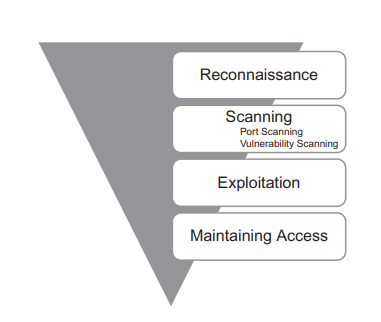
\includegraphics[scale=1]{\imagedir/Phasen_eines_Pentests.png}
	\caption{Phasen eines Penetrationtests}
	\label{Phasen eines Penetrationtests} \cite{B1}
\end{figure}

Das in der Abbildung 1.1 abgebildete Dreieck symbolisiert dabei, dass eine breit angesammelte Menge an Informationen kombiniert mit der passenden Abstraktion über die weiteren Phasen schließlich zu einem erfolgreichen Pentest führt. 

Der zweite Schritt, das Scanning, kann in zwei weitere Bestandteile aufgeteilt werden. Mit den in der Reconnaissance herausgefundenen IP-Adressen kann nun ein Port-Scan durchgeführt werden, um offene Ports und potentielle Services zu identifizieren. \cite{B2} \\
Als nächstes wird das Vulnerability Scanning ausgeführt. Dabei werden Schwachstellen in der Software und in den Services des Zielsystems lokalisiert und identifiziert. \cite{B3}

!! Den Text hier unten nochmal durchchecken, der ist später dazu gekommen !!

Anhand der Ergebnisse unserer Scans können wir nun mit der Exploitation-Phase, also der Ausnutzung von Schwachstellen beginnen. 
Da wir nun genau wissen welche Ports und Services Angriffsfläche bieten und sogar die Schwachstellen kennen, können wir nun beginnen unser Zielsystem systematisch anzugreifen. \cite{B1}\\
Beim exploiting gibt es zahlreiche Ansätze und Vorgehensweisen. Hauptziel ist jedoch immer, Zugriff auf das Zielsystem zu erlangen und seine Zugriffsrechte auf dem System so zu eskalieren, dass man Administratorrechte auf dem Zielsystem erlangt. \cite{B4}

Die letzte Phase die durchschritten wird ist die Maintaining Access Phase. Haufig wird bei einer Ausnutzung einer Schwachstellen nur temporärer Zugriff auf das Zielsystem möglich. \\
Da viele Sicherheitslücken keinen dauerhaften Zugriff erlauben, wird während des temporären Zugriffs im Zielsystem versucht, eine weiter Möglichkeit zu schaffen auf das Zielsystem zu gelangen. \cite{6}

Formal wird einem Pentest in der Regel noch eine letzte Phase, das Reporting hinzugefügt, an welchem oftmals die Qualität eines Pentests gemessen wird.
Ein Report beinhaltete alle relevanten Informationen über den vollzogenen Pentest. 
Hierbei werden Sicherheitslücken aufgedeckt und an den nötigen Stellen wird zusätzlich erläutert, welche Schritte im Pentest stattgefunden haben. 
Gegebenenfalls werden vom Pentester noch Vorschläge gemacht, wie die Sicherheitslücken ausgebessert werden können. \cite{B1}

\section{XY}

Weiterer wissenschaftlicher Input zu Schwachstellen in Web Applikationen z.B. OWASP top 10



% !TEX root =  master.tex
\chapter{Auswahl der Tools und der Umgebung}

In diesem Kapitel ...

- Hier kurz einmal Erklären welche Tools verwendet werden und evtl. 1-2 Sätze zu jedem.

- Erläutern wie nach welchen Kriterien die Tools verglichen werden

- Erläutern, dass der Juice Shop als Zielsystem verwendet wird. Oder doch vlt WAVSEP ? - WAVSEP Ist denke ich bessser, weils extra dafür gemacht ist + eine umfangreichere Sammlung an Schwachstellen hat
https://github.com/sectooladdict/wavsep
\url{https://owasp.org/www-project-benchmark/}

http://projects.webappsec.org/w/page/13246986/Web%20Application%20Security%20Scanner%20Evaluation%20Criteria

\url{https://norma.ncirl.ie/4165/1/mandarprashantshah.pdf}


Scanner: nmap, sslscan, nikto
nmap
sslscan
fuff
sql map
nikto
nuclei
burp community,
metasploit

Unterschiedung Kategorisierung der Tools

wstg owasp, vergleichbar gegenüber halten


\section{Testkriterien}

Um die Auswertung und Validierung der Tests möglichst strukturiert zu gestalten werden nachfolgend Kriterien festgelegt, nach denen die einzelnen Tools und Techniken verglichen werden.
Hierfür werden bereits vorhandene und gängige Kriterien mit zusätzlich weiteren wichtigen Kriterien kombiniert.

Paar Kriterien (Brainstorming):
\url{https://norma.ncirl.ie/4165/1/mandarprashantshah.pdf}
\begin{itemize}
	\item \textbf{(Scanning) Speed} 
	\item \textbf{Vulnerability Detection Rate} 
	\item \textbf{True Positive and False Positive reported} 
	\item \textbf{Einfache Bedienung und Nachvollziehbarkeit} \\
	dd
\end{itemize}



\subsection{OWSAP Benchmark test}
Der OWASP Benchmark test ist eine Java basierte open source Tetsumgebung zur Erkennung von Schwachstellen.
OWASP benchmark ist eine bewährte Testumgebung, die regelmäßig geupdatet wird. Die Testumgebung umfasst dabei über 2740 potentielle Schwachstellen.

Um den Testdurchlauf möglichst strukturiert und systematisch zu gestalten, werden nachfolgend Kriterien aufgestellt, nach denen die einzelnen Tools und Techniken verglichen werden. 

In den bisherigen Abschnitten dieser Arbeit haben wir uns bereits mit den Grundlagen von Pentesting, sowie der generellen Vorgehensweisen und Pentesting Frameorks beschäftigt. 
Unter zahlreichen möglichen Zielsystem hat sich das Framework OWASP Benchamrk zum Testen und Vergleichen verschiedener Pentesting Tools als sehr geeignet bewährt.
OWASP Benchmark bietet dazu zahlreiche Testcases und wird immernoch aktiv geupdatet. 

Eines dieser Frameworks

\section{Auswahl der Tools}

Kategorisierung: In dieser Arbeit werden 


\section{Zielsystem}

Um die Zuverlässigkeit während dem Vergleich der einzelnen Tools zu gewährleisten, ist es wichtig die richtige Testumgebung zu wählen. 
Nachfolgend werden einige Kriterien beschrieben, die eine passende Testumgebung benötigt:

\begin{itemize}
	\item \textbf{Umfassende Abdeckung} \\
	Die Testumgebung sollte eine Vielzahl bekannter Schwachstellen und Angriffsszenarien bereitstellen, um ein umfassendes Testen der Tools zu ermöglichen.
	\item \textbf{Konsistenz} \\
	Damit die Unterschiede, sowie Vor- und Nachteile der einzelnen Tools aufgedeckt werden können, sollte die Testumgebung möglichst einheitliche Verfahren und Messmethoden bereitstellen.
	\item \textbf{Realitätsnähe} \\
	Die zu untersuchenden Tools begleiten zahlreiche Pentester täglich in realen Szenarien.
	Daher sollen die in der Testumgebung bereitgestellten Angriffsszenarien und Schwachstellen möglichst realitätsnah sein. 
	\item \textbf{Einfache Bedienung und Nachvollziehbarkeit} \\
	Die Testumgebung sollte eine einfache Bedingung und eine Dokumentation bereitstellen um eine schnelle und problemlose Verwendung zu ermöglichen.
	Außerdem sollten die Ergebnisse und Methodiken seitens der Testumgebung nachvollziehbar sein.
\end{itemize}

Aufgrund der aufgestellten Kriterien wird das Web Application Vulnerability Scanner Evaluation Project (WAVSEP) als adäquate Testumgebung gewählt. WAVSEP ist eine bewährte Testumgebung, die auf den Vergleich von Pentestools ausgelegt ist.  \\
Dabei bietet WAVSEP ein umfassendes Set an passende Angriffsszenarien, die optimale Bedingungen schaffen, um die Genauigkeit und Zuverlässigkeit von Pentesttools direkt miteinander zu vergleichen.
Dabei verwendet WAVSEP einheitliche und nachvollziehbare Messmethoden, die den direkten Vergleich einzelner Tools erleichtern. \\
WAVSEP ist daher eine hervorragende Wahl für die Bewertung von Penetrationstools.

\section{Testumgebung}
Die Durchführung der Tests findet auf einer Kali Linux VW mit einer Windows host Maschine statt. 
Um das Testen zu ermöglichen muss zunächst alle nötige Software installiert werden, um das Zielsystem schließlich angreifen zu können


% !TEX root =  master.tex
\chapter{Analyse}

In diesem Kapitel ...

% !TEX root =  master.tex
\chapter{Schwachstellenerkennung unter Verwendung von künstlicher Intelligenz}

In diesem Kapitel:

- kurzer allgemeiner Text, über das Thema

- Beschreibung/Erklärung von http://repository.kpi.kharkov.ua/handle/KhPI-Press/54956

- Etwas über zukunftsfähigkeit und Vorteile/Nachteile schreiben

Bevor in Kapitel sechs eine audäquate Evaluierung und Auswertung stattfinden soll, wird vorher noch eine weitere Methodik/Technik untersucht, die unter Verwendung von künstlicher Intelligenz Schwachstellen erkennt und versucht diese auszunutzen. 
Diese Methodik gilt im Vergleich zu den bisher vorgestellten Tools und Techniken zu den eher jüngeren Technologien.





% !TEX root =  master.tex
\chapter{Evaluierung und Auswertung}

In diesem Kapitel ...

- Auswertung der Anlalyseergebnisse 

- Vergleiche zwischen den Tools

- Vergleiche zwischen manuell und automatisiert

- Vor und Nachteile einzelner Dinge

- Rückschlüsse ziehen auf die vorherigen Kapitel




% Fazit und Ausblick
% !TEX root =  master.tex
\chapter{Abschluss}





%%%%%%%%%%%%%%%%%%%%%%%%%%%%%%%%%%%

%%%%%%%%%%%%%%%%%%%%%%%%%%%%%%%%%%%
% ANHÄNGE
%
% @stud: einzelne Anhänge bearbeiten und eigene Anhänge hier einfügen 
%        die nachfolgenden Zeilen deaktivieren, wenn keine Anhänge verwendet werden
%
\initializeAppendix
% !TEX root =  master.tex
\chapter{Literaturverzeichnis}

	\textbf{[B1] Engebretson, P. (2013).
	The basics of hacking and penetration testing: ethical hacking and penetration testing made easy. Elsevier.} \\
	\url{http://dspace.fudutsinma.edu.ng/xmlui/bitstream/handle/123456789/845/ebooksclub.org__The_Basics_of_Hacking_and_Penetration_Testing__Ethical_Hacking_and_Penetration_Testing_Made_Easy.pdf?sequence=1}
	
	
	\textbf{[B2] Yaworski, P. (2018): Web Hacking 101. No Starch Press.} \\
	\url{https://digtvbg.com/files/books-for-hacking/Web%20Hacking%20101%20-%20How%20to%20Make%20Money%20Hacking%20Ethically%20by%20Peter%20Yaworski.pdf}
	
	\textbf{[B3] Mastering Defensive Security by Cesar Bravo, Darren Kitchen.} \\
	\url{https://learning.oreilly.com/library/view/mastering-defensive-security/9781800208162/B16290_FM_Final_JC_ePub.xhtml}
	
	\textbf{[B4] Penetration Testing - A Hands-On Introduction to Hacking}
	


\section{Quellenerzeichnis}

	\textbf{[1] Siemens Indusrty Software Inc.} \\
	Intelligentere Entscheidungen, bessere Produkte durch umfassendes PLM \\
	\url{https://www.plm.automation.siemens.com/de_de/Images/tc_overview_tcm73%-62348.pdf}
	
	\textbf{[2] Cost of data breach 2022} \\
	\url{https://www.ibm.com/reports/data-breach}
	
	\textbf{[3] Patrick Engebretson "The Basics of hacking
		and penetration testing"} \\
	\url{http://dspace.fudutsinma.edu.ng/xmlui/bitstream/handle/123456789/845/ebooksclub.org__The_Basics_of_Hacking_and_Penetration_Testing__Ethical_Hacking_and_Penetration_Testing_Made_Easy.pdf?sequence=1}
	
	\textbf{[4] Deep Learning und Pentesting} \\
	\url{http://repository.kpi.kharkov.ua/handle/KhPI-Press/54956}
	
	\textbf{[5] CHIEM TRIEU PHONG, A Study of Penetration Testing Tools
		and Approaches} \\
	\url{https://openrepository.aut.ac.nz/bitstream/handle/10292/7801/ChiemTP.pdf?sequence=3&isAllowed=y}
	
	\textbf{[6] A Study on Penetration Testing Process and Tools } \\
	\url{https://ieeexplore.ieee.org/stamp/stamp.jsp?arnumber=8378035&casa_token=XNKWbXqAGogAAAAA:zi_TswzVWQeWmdEiCATwmOxCQ_L8-exnSsgQQQBM3ahGCG2iCg5ciNeyWkrBJxe6sdI7n4ycT11MBEY&tag=1}
	
	\textbf{[7] Shah, M. P. (2020). Comparative analysis of the automated penetration testing tools (Doctoral dissertation, Dublin, National College of Ireland).} \\
	\url{https://norma.ncirl.ie/4165/1/mandarprashantshah.pdf}
	
	\textbf{[8] Penetration Testing in a Web
		Application Environment} \\
	\url{http://www.diva-portal.org/smash/get/diva2:356502/fulltext01.pdf}
	
	Das hier später noch Aufräumen und Citavi oder so verwedent
	
	weitere Quellen
	
	\url{https://sectooladdict.blogspot.com/}
	
	\url{https://owasp.org/www-community/Vulnerability_Scanning_Tools}
	
\section{Bildverzeichnis}


\begin{figure}[H]
	\centering 
	\frame{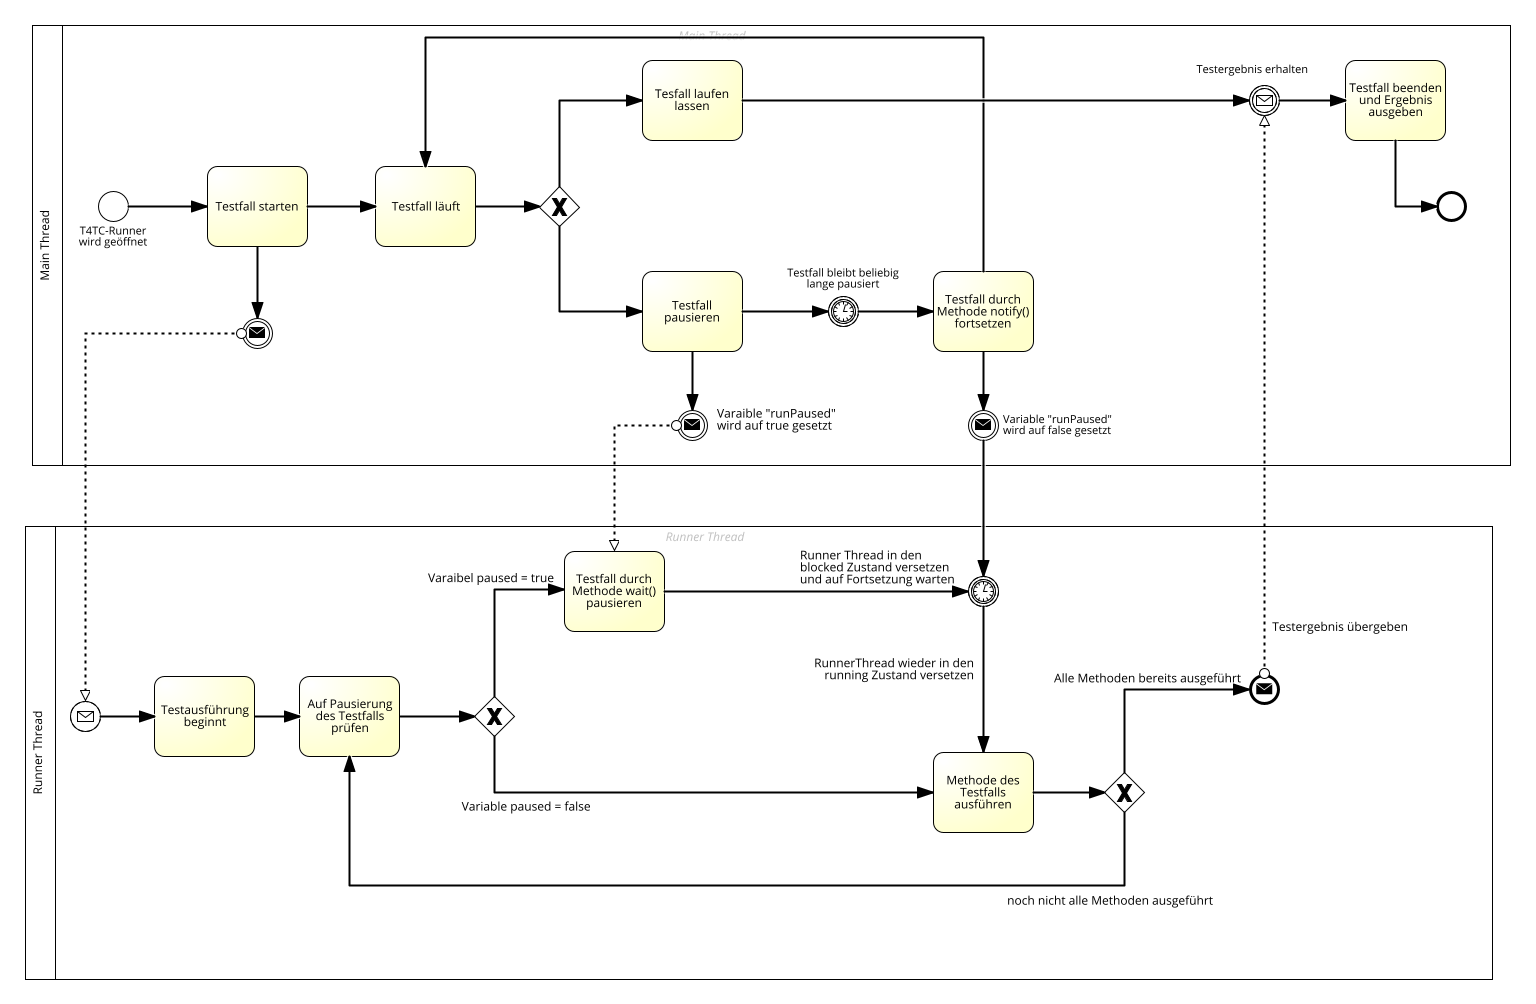
\includegraphics[scale=0.6, angle=90]{\imagedir/Pause-function (3).png}}
	\caption{vereinfachtes Prozessdiagramm der neuen Testausführung} \cite{Quelle: eigene Darsetllung}
	\label{BPMN}
\end{figure}

% !TEX root =  master.tex

%%%%%%%%%%%%%%%%%%%%%%%%%%%%%%%%%%%

\singlespacing

%%%%%%%%%%%%%%%%%%%%%%%%%%%%%%%%%%%
% LITERATURVERZEICHNIS
% @stud: Literaturverzeichnis in Datei bibliography.bib anpassen. 
%
% Alternative zu Verwendung von \initializeBibliography: Citavi ...
% (dann \initializeBibliography auskommentieren und eigenes LaTex Coding verwenden)
%
\initializeBibliography
%%%%%%%%%%%%%%%%%%%%%%%%%%%%%%%%%%%

%%%%%%%%%%%%%%%%%%%%%%%%%%%%%%%%%%%
% INDEX
% @stud: ggf. Index auskommentieren, wenn nicht benötigt
%
\addcontentsline{toc}{chapter}{Index}
\printindex

\end{document}
